

%\def\myarray{{"blue!05", "blue!20", "blue!40"}}
\def\myarray{{"blue!10", "blue!10", "blue!10"}}
\def\xk{0.3}
\def\yk{0.2}
\def\xs{0.9}
\def\ys{0.8}
\def\xl{1.5}
\def\yl{1.5}

 \def\dia{0.5em}
 \def\dist{1.5}
 \def\xnull{0.3}
 \def\ynull{0.2}

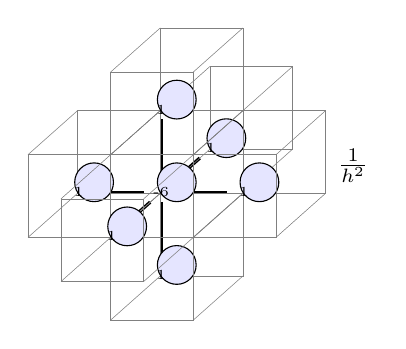
\begin{tikzpicture}[scale=0.7]
 \node  (M) at (\xnull,\ynull) {\makebox[\dia]{}};

 \node  (T) at (\xnull,\ynull+\dist) {\makebox[\dia]{}};
 \draw[very thick] (M) -- (T);

 \node (Bo) at (\xnull,\ynull-\dist) {\makebox[\dia]{}};
 \draw[very thick] (M) -- (Bo);

 \node (L) at (\xnull-\dist,\ynull) {\makebox[\dia]{}};
 \draw[very thick] (M) -- (L);

 \node  (R) at (\xnull+\dist,\ynull) {\makebox[\dia]{}};
 \draw[very thick] (M) -- (R);

 \node  (F) at (\xnull-\xs,\ynull-\ys) {\makebox[\dia]{}};
 \draw[very thick] (M) -- (F);

 \node  (Ba) at (\xnull+\xs,\ynull+\ys) {\makebox[\dia]{}};
 \draw[very thick] (M) -- (Ba);

\ifnum1=1 % auf =0 setzen, um das Gitter auszublenden
\foreach \z in {-1, 0,1} {
  \foreach \x in {-1, 0,1} {
    \pgfmathmultiply{\z}{\xs}
    \let\xshift\pgfmathresult
    \pgfmathmultiply{\x}{\xl}
    \pgfmathsubtract{\pgfmathresult}{\xshift}
    \let\xnull\pgfmathresult
    \foreach \y in {-1, 0,1} {
      \pgfmathparse{(\x==0 && \y==0) || (\x==0 && \z==0) || (\z==0 && \y==0) ?int(1):int(0)}
      \ifnum\pgfmathresult>0\relax
      \pgfmathmultiply{\z}{\ys}
      \let\yshift\pgfmathresult
      \pgfmathmultiply{\y}{\yl}
      \pgfmathsubtract{\pgfmathresult}{\yshift}
      \let\ynull\pgfmathresult
      \draw[very thin,gray] (\xnull,\ynull) -- (\xnull,\ynull+\yl) -- (\xnull+\xl,\ynull+\yl) -- (\xnull+\xl,\ynull) -- cycle;
      \draw[very thin,gray] (\xnull-\xs,\ynull-\ys) -- (\xnull,\ynull);
      \draw[very thin,gray] (\xnull+\xl-\xs,\ynull-\ys) -- (\xnull+\xl,\ynull);
      \draw[very thin,gray] (\xnull-\xs,\ynull+\yl-\ys) -- (\xnull,\ynull+\yl);
%        \pgfmathparse{\myarray[\z+1]}
%        \draw[fill=\pgfmathresult] (\xk+\xnull,\yk+\ynull) circle (1em);
      \draw[fill=blue!10] (\xk+\xnull,\yk+\ynull) circle (1em);
%      \node [circle,draw,fill=blue!10]  at (\xk+\xnull,\yk+\ynull)  {\makebox[\dia]{}};
      \draw[very thin,gray] (\xnull+\xl-\xs,\ynull+\yl-\ys) -- (\xnull+\xl,\ynull+\yl);
      \draw[very thin,gray] (\xnull-\xs,\ynull-\ys) -- (\xnull-\xs,\ynull-\ys+\yl) -- (\xnull-\xs+\xl,\ynull-\ys+\yl) -- (\xnull-\xs+\xl,\ynull-\ys) -- cycle;
      \fi
    }
  }
}
\fi

 \node at (M)  {\tiny -6};
 \node at (T)  {\tiny 1};
 \node at (Bo) {\tiny 1};
 \node at (L) {\tiny 1};
 \node at (R) {\tiny 1};
 \node at (F) {\tiny 1};
 \node at (Ba) {\tiny 1};

 \node at (3.5,0.5) { $ \frac{1}{h^2} $ };
\end{tikzpicture}
